% \textbf{Title: Sampling 4}

Consider a signal with this spectrum.

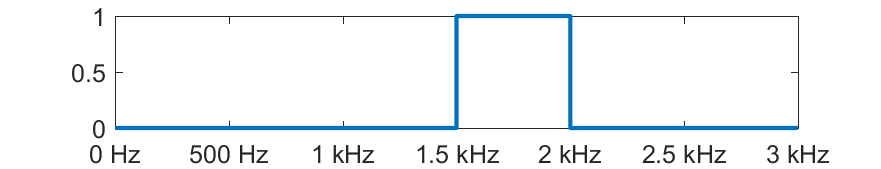
\includegraphics[width=4.60233in,height=0.88285in]{../../Images/SamplingAndAliasingQ4.png}

Which sampling frequency \(f_{s}\) could we use if we want to reconstruct the signal with an ideal high-pass filter? \\

a. \(f_{s} = 2\ kHz\).

%@ Incorrect. This question tests the concept ``Sampling and Aliasing'', which is taught in these courses.

b. \(f_{s} = 4\ kHz\).

%@ Incorrect. This question tests the concept ``Sampling and Aliasing'', which is taught in these courses.

c. \(f_{s} = 48\ kHz\).

%@ Incorrect. This question tests the concept ``Sampling and Aliasing'', which is taught in these courses.

*d. The signal cannot be reconstructed.

%@ Correct! This question tests the concept ``Sampling and Aliasing'', which is taught in these courses.

e. I do not know. \\

%@ It's okay. This question tests the concept ``Sampling and Aliasing'', which is taught in these courses.
